%%%%%%%%%%%%%%%%%%%%%%%%%%%%%%%%%%%%%%%%%%%%%%%%%%%%%%%%%%%%%%%%%%%%%%%%
%%
%% template.tex
%% このサンプルは,LaTeX-2e 専用です。
%%                      
%% Change Log
%% 2010-04-19 Yasuhiro Sugimoto <yas@mech.eng.osaka-u.ac.jp>
%% * 大須賀・石川研研究会資料用に修正
%%
%% 2018-1-1 Keisuke Naniwa <naniwa@es.hokudai.ac.jp>
%% * 大須賀・杉本研研究会資料用に修正
%%   osukaLab2018.styを使用することを前提にした記述とパッケージに変更
%%  いくつかのべからず集を記載してあるので,熟読の上資料作成のこと(ここすら読んでないなら知らん)
%%
%%  $Id: template.tex,v 1.2 2000/01/12 08:18:03 ken Exp $
%%
%%%%%%%%%%%%%%%%%%%%%%%%%%%%%%%%%%%%%%%%%%%%%%%%%%%%%%%%%%%%%%%%%%%%%%%%
\documentclass[a4j]{jsarticle}
\usepackage{osukalab2018}%使用前にstyファイル内を一度目を通しておくこと
\usepackage{epic,eepic}
\usepackage[dvipdfmx]{graphicx}
\usepackage{amsmath}	% required for `\align' (yatex added)もし必要なパッケージがインクルードされてない場合,こんな感じでやてふが自動で入れてくれます(ただし^C^Bでやった場合だけ.みんな^C^B使ってるよね・・・?)

%\usepackage{epsfig} % このパッケージは使わずに画像の形式はPDFを使いましょう
%写真はjpg,スクショはpng,グラフやイラストはpdfで
%matlabでのグラフ出力については別で
\usepackage{siunitx} %単位や数値が綺麗に入ります
%\usepackage{times} % これもう古いのでtxfonts使おね
\usepackage{txfonts} %綺麗なtimesフォント系への切り替え
\usepackage{amssymb}
\usepackage{cite}

\usepackage{url}%url記入したかったので使用,普段はいらないはず


\pagestyle{empty}

\headding{大須賀・杉本研 研究会資料}
% 和文題名
\title{大須賀・石川研 研究会資料用スタイルファイル}  
% 英文題名
%\etitle{p\LaTeX-Style file for Osuka-Sugimoto Lab. Meeting}
% 著者の和文名
\author{
     浪花 啓右
     }
% 著者の英文名
%\engauthor{
%     Keisuke NANIWA
%}
% 英文の概要
\abstract{Please write your English abstract here.
}
% キーワード
\keywords{研究会資料,大須賀・石川研,大阪大学}
%

\begin{document}
\maketitle
\thispagestyle{empty}
%
\section{はじめに}
以下に色々な例示をします.
ソースファイルと出力の関係をしっかり理解しましょう.
一部スタートダッシュ課題の解答に近いものや,解答そのものがあるので,スタートダッシュプログラムを終えてから参照する方が良いかもしれません.

\section{いろんな基本}
\subsection{文章での基本}
分野や流派によって異なりますが,基本的に句読点はカンマとピリオドを使用しましょう.
日本語の文中では,カンマとピリオドは全角,数式や英文の中では半角で記入しましょう.
また,一部漢字をなるべく使わないなどのマナーもあります.(ex.殆ど→ほとんど,最も→もっとも,など)漢字使うとかっこいいかもしれませんが,ぶっちゃけ読みづらいです(逆もまたしかりですが,あまりにもひらがなばかりだと読みにくい場合もありますよね).大切なのは指定のルールに従うことと,ルールに記載がなければあなたの采配で,資料や論文内で統一することです.
漢字かひらがなか迷ったらこちらのサイトなどを参照するのも良いでしょう.

\url{http://www.yamanouchi-yri.com/yrihp/techwrt-2-4s/t-2-4s03a.htm}


また,改行ですが\\
この方法は使わずに

このように空行を入れることで改行するようにしましょう.なぜかは出力を見ればわかるはずです.スラッシュによる改行はtabler環境内だけなどにしましょう.

また,たまに太字やイタリックを使いたくなることはあるでしょうが,{\bf このやり方や,}{\it Such a method}はやめましょう.\textbf{こちらのやり方や,}\textit{Such a method}を使いましょう.

\subsection{数式での基本}

数式はカギカッコもしくはalign環境で書きましょう.短く$5.0$~Vとか書きたければこんな感じで.ちなみに具体的な数字の場合は単位に括弧はつけずに,$x$~(m)とか文字の場合は括弧をつけるのがスタンダードだと思っています.単位の前には改行されない半角スペースを入れるのも忘れずに.\si{kg.m.s^{-1}}とかの単位も,\num{3.14159265e34}とか\num{.3e45}の数字もsiunitパッケージ入れてると綺麗にかけるよね.数字のリストもサポートしてくれているので\numlist{ 1.0; 2.0; 3.0; 4.0; 5.0}とか,\SIlist{ 1.0; 2.0; 3.0; 4.0; 5.0}{\volt}なんてこともできるね!でもこれ英語での場合だね.あまり気にしなくてもいいかもね.

数式は式番号いらないなら
\[
 y=\sin{A}
\] 
式番号がいるなら
\begin{align}
 y=\sin{A}
 \label{eq:test}
\end{align}
どちらの環境内でも最新のやてふなら数学記号のショートカット(セミコロンキー)やギリシャ文字のショートカット(コロンキー)に反応してくれるので安心です.
式を参照する場合は\refeq{test}とするとOK.

\subsection{図の基本}

スーパー何度も書いたり言ったりしてるのでさすがに大丈夫だと思いますが,
\begin{itemize}
 \item グラフや図,線描のイラストはベクタ画像であるpdf形式で
 \item 写真などはラスタ画像であるjpgで
 \item スクリーンショットはD2D(dot to dot)の画像データになるのでpngで
\end{itemize}
載せましょう.これら全ては最終出力となる書類のpdfに直接埋め込むことができるので,タイプセットも早くて楽です.

%図の引用の例~\ref{fig:test}これは間違いではないけど・・・
図の引用の例~\reffig{test}.%せっかくreffigあるので活用しましょう.


\begin{figure}[tb]
 \centering %center環境はズレやすいから使わないこと
  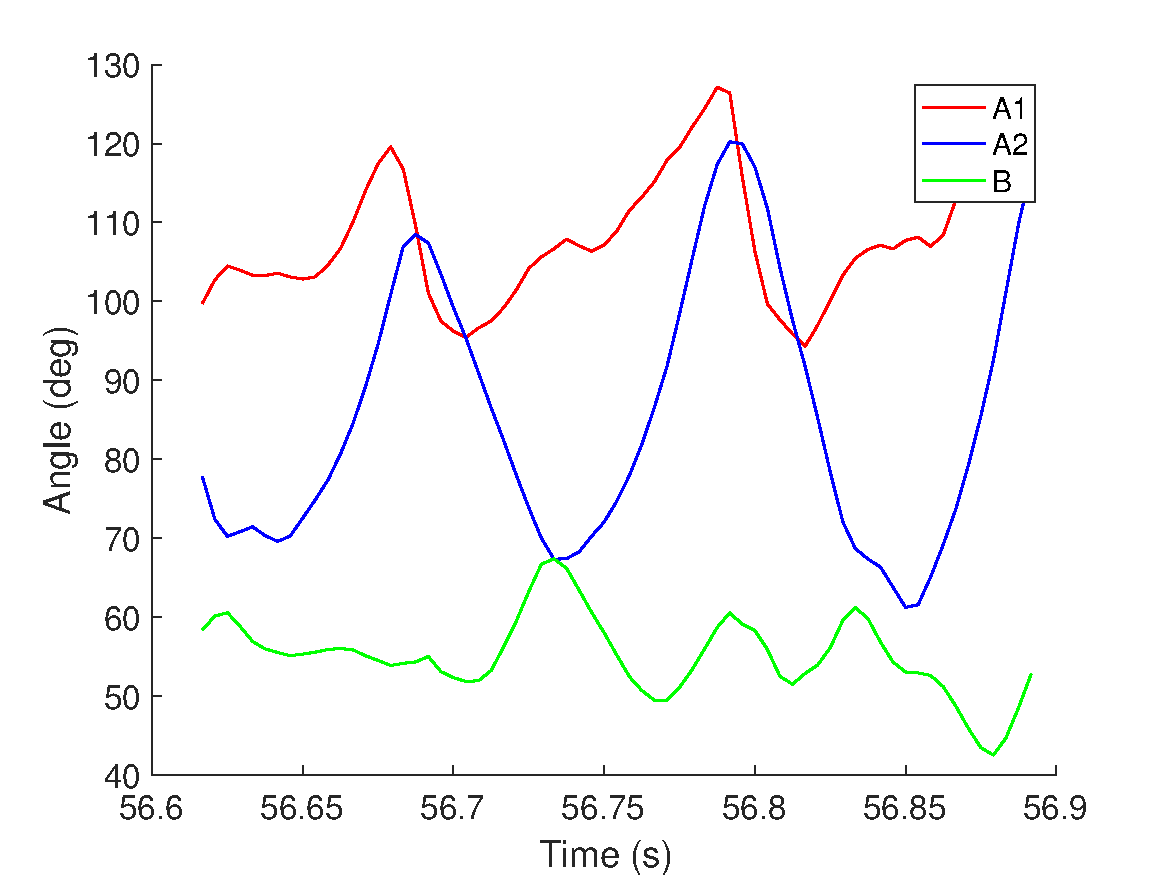
\includegraphics[width=\columnwidth]{./figure/testfig.pdf}
  \caption{Test 1}
  \label{fig:test}
\end{figure}

\begin{figure}[tb]
 \centering %center環境はズレやすいから使わないこと
  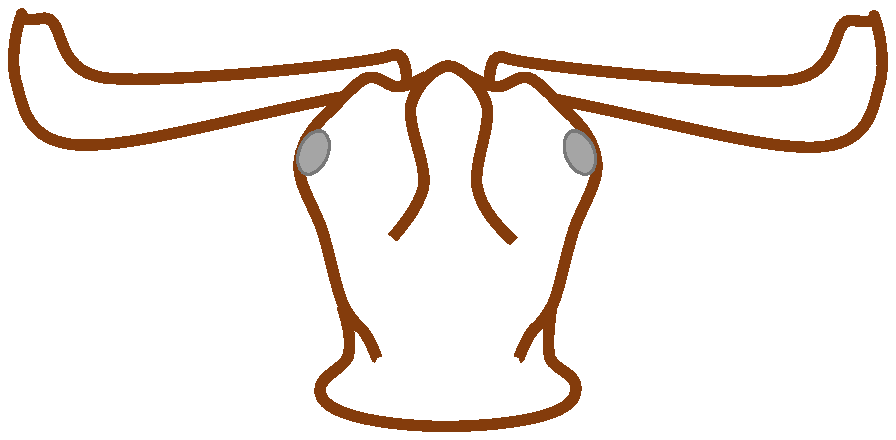
\includegraphics[width=\columnwidth]{./figure/testfig2.pdf}
  \caption{Test 2}
  \label{fig:test2}
\end{figure}

\begin{table*}[t!]
  \caption{Sample table}
   \label{table:test}
   \centering
   \begin{tabular}{cccccr}\hline
    Type & Name & Voltage & Unit & This is sample & by keisuke naniwa\\ \hline \hline
   Exp. A & 46\%& 33\%& 21\%& --& --\\ \hline
   Exp. B & 64\%& 9\%& 27\%& 60\%& 13\%\\ \hline    
   \end{tabular}
\end{table*}




参考文献の例~\cite{mike,bibtest}.



  
\section*{謝辞とか}
%
% 以下に文献を書きます。
%
{\small
\bibliographystyle{osukalab}
\bibliography{myref}


\clearpage

\end{document}

